\documentclass{article}
\usepackage[utf8]{inputenc} %кодировка
\usepackage[T2A]{fontenc}
\usepackage[english,russian]{babel} %русификатор 
\usepackage{mathtools} %библиотека матеши
\usepackage[left=1cm,right=1cm,top=2cm,bottom=2cm,bindingoffset=0cm]{geometry} %изменение отступов на листе
\usepackage{amsmath}
\usepackage{graphicx} %библиотека для графики и картинок
\graphicspath{}
\DeclareGraphicsExtensions{.pdf,.png,.jpg}
\usepackage{subcaption}
\usepackage{pgfplots}
\usepackage{listings}
\usepackage{derivative}
\pgfplotsset{compat=1.16}

\begin{document}
% НАЧАЛО ТИТУЛЬНОГО ЛИСТА
\begin{center}
    \Large
    Федеральное государственное автономное \\
    образовательное учреждение высшего образования \\ 
    «Научно-образовательная корпорация ИТМО»\\
    \vspace{0.5cm}
    \large
    Факультет программной инженерии и компьютерной техники \\
    Направление подготовки 09.03.04 Программная инженерия \\
    \vspace{1cm}
    \Large
    \textbf{Отчёт по лабораторной работе №2} \\
    По дисциплине «Вычислительная математика» (четвёртый семестр)\\
    \large
    \vspace{8cm}

    \begin{minipage}{.33\textwidth}
    \end{minipage}
    \hfill
    \begin{minipage}{.4\textwidth}
    
        \textbf{Студент}: \vspace{.1cm} \\
        \ Дениченко Александр P3212\\
        \textbf{Практик}:  \\
        \ Наумова Надежда Александровна
    \end{minipage}
    \vfill
Санкт-Петербург\\ 2024 г.
\end{center}

% КОНЕЦ ТИТУЛЬНОГО ЛИСТА 
\newpage
\begin{center}
    \LARGE
    \color{pink}
    \LaTeX \color{lime}.
\end{center}

\section{Цель работы}

Изучить численные методы решения нелинейных уравнений и их
систем, найти корни заданного нелинейного уравнения/системы нелинейных уравнений,
выполнить программную реализацию методов.


\section{Задание}
Часть 1.

1. Отделить корни заданного нелинейного уравнения графически (вид уравнения представлен в табл. 6)

2. Определить интервалы изоляции корней.

3. Уточнить корни нелинейного уравнения (см. табл. 6) с точностью $\epsilon=10^{-2}$.

4. Используемые методы для уточнения каждого из 3-х корней многочлена
представлены в таблице 7.

5. Вычисления оформить в виде таблиц (1-5), в зависимости от заданного метода. Для всех значений в таблице удержать 3 знака после запятой.

5.1 Для метода половинного деления заполнить таблицу 1.

5.2 Для метода хорд заполнить таблицу 2.

5.3 Для метода Ньютона заполнить таблицу 3.

5.4 Для метода секущих заполнить таблицу 4.

5.5 Для метода простой итерации заполнить таблицу 5. Проверить условие сходимости метода на выбранном интервале.

6. Заполненные таблицы отобразить в отчете.
\\ \\
Вид нелинейного уравнения для вычислительной реализации:
\[
    3x^3+1,7x^2-15,42x+6,89\]
Выбор метода для вычислительной реализации задачи:
\begin{table}[h]
    \centering
    \begin{tabular}{|*{4}{c|}}
        \hline
        Номер & Крайний & Крайний & Центральный  \\
        варианта & правый корень & левый корень & корень \\
        \hline
        8 & Метод простой итерации (5) & Метод хорд (2) & Метод Ньютона (3) \\
        \hline
    \end{tabular}
    \caption{Методы для вычислительной реализации}
\end{table}

\section{Выполнение первой части}
Точки пересечения:

\[x_3(1.67953,0)\] 
\[x_2(0.498258,0)\] 
\[x_1(-2.7445,0)\]
Построим график функции:
\begin{center}
    \begin{tikzpicture}
        \begin{axis}[
            xlabel={$x$},
            ylabel={$y$},
            xmin=-4, xmax=4,
            ymin=-10, ymax=30,
            axis lines=middle,
            grid=both,
            samples=1000,
            domain=-4:4,
            thick,
            legend style={at={(0.5,-0.15)},anchor=north}
        ]
        
        \addplot[blue] {3*x^3 + 1.7*x^2 - 15.42*x + 6.89};
        \addlegendentry{$3x^3 + 1.7x^2 - 15.42x + 6.89$}
        % Находим корни уравнения
        \draw[fill=black] (1.67953,0) circle [radius=2pt] node[below] {$x_3$};
        \draw[fill=black] (0.498258,0) circle [radius=2pt] node[below] {$x_2$};
        \draw[fill=black] (-2.7445,0) circle [radius=2pt] node[below] {$x_1$};
        
        \end{axis}
        \end{tikzpicture}
\end{center}
\textbf{1. Метод простой итерации для $x_3(1.67953,0)$.}

\begin{center}
    \begin{tikzpicture}
        \begin{axis}[
            xlabel={$x$},
            ylabel={$y$},
            xmin=1.1, xmax=2,
            ymin=-5, ymax=2,
            axis lines=middle,
            grid=both,
            samples=500,
            domain=-4:4,
            thick,
            legend style={at={(0.5,-0.15)},anchor=north}
        ]
        
        \addplot[blue] {3*x^3 + 1.7*x^2 - 15.42*x + 6.89};
        \addlegendentry{$3x^3 + 1.7x^2 - 15.42x + 6.89$}
        % Находим корни уравнения
        \draw[fill=black] (1.67953,0) circle [radius=2pt] node[below] {$x_3$};
        \draw[fill=black] (0.498258,0) circle [radius=2pt] node[below] {$x_2$};
        \draw[fill=black] (-2.7445,0) circle [radius=2pt] node[below] {$x_1$};
        
        \end{axis}
        \end{tikzpicture}
\end{center}

Приведём уравнение:
\[
    3x^3+1,7x^2-15,42x+6,89 = 0 \]
к следующему виду:
\[x = \phi (x)\]
получим:
\[
    \phi (x) = 0,195x^3+0,110x^2+0,447 = 0 \]
    \[
    \phi' (x) = 0,585x^2+0,220x \]
Пусть начальное приближение будет:
\[
    a_0 = 1,2;\ b_0 = 2\]
Тогда проверим условие сходимости:
\[
    \phi' (1,2) = 0,805 < 1 \]
    \[
    \phi' (2) = 0,585\cdot 4+0,220\cdot 2 = 2,34+0,44 = 2,78 > 1 \]
\[
    q = max_{[a,b]}|\phi'(x)| = 2,78 > 1
\]
Сходимости нет.
\\ \\
Пойдём по другому способу, где применяется приём введения параметра $\lambda$:
\[
    f(x) = 3x^3+1,7x^2-15,42x+6,89 \]
\[\lambda f(x) = 0\ (\lambda!=0)\]
\[\phi(x)\ = x+ \lambda f(x) \]
\[\phi'(x)\ = 1+ \lambda f'(x) \]
\[f'(x) = 9x^2 +3,4x - 15,42\]
\[f'(1,2) = 9\cdot (1,2)^2 +3,4\cdot (1,2) - 15,42 = 1,62\]
\[f'(2) = 9\cdot 4 +3,4\cdot 2 - 15,42 = 27,38\]
Так как $f'[a, b] > 0$, то рассматриваем:
\[
    \lambda = - \frac{1}{max|f'(x)|} = -\frac{1}{27,38} = -0,037\] 
Подставим:
\[\phi(x) = x -0,037 \cdot (3x^3+1,7x^2-15,42x+6,89)= \] 
\[= 1,571x - 0,111x^3 - 0,063x^2 - 0,255\]
\[\phi'(x) = 1,571 - 0,333 x^2 - 0,126x\]
Проверим точки:
\[\phi'(1,2) = 1,571 - 0,333\cdot(1,2)^2 - 0,126\cdot 1,2 = 0,940 < 1\]
\[\phi'(2) = 1,571 - 0,333\cdot(2)^2 - 0,126\cdot 2 = -0,013 < 1\]
Условие сходимости выполняется!
\[x_0 = 1,2 \]
\[x_1 = \phi(x_0) = 1,571\cdot 1,2 - 0,111\cdot(1,2)^3 - 0,063\cdot(1,2)^2 - 0,255 = 1,348\]
\[x_2 = 1,571\cdot 1,348 - 0,111\cdot(1,348)^3 - 0,063\cdot(1,348)^2 - 0,255 = 1,476\] 
\[f(x_2) = 3\cdot (1,476)^3+1,7\cdot (1,476)^2-15,42\cdot (1,476)+6,89 = -2,520\]
...
\[
    f(x) = 3x^3+1,7x^2-15,42x+6,89 \]
\[\phi(x)= 1,571x - 0,111x^3 - 0,063x^2 - 0,255\]


\begin{table}[h]
    \centering
    \begin{tabular}{|*{6}{c|}}
        \hline
        Номер & $x_i$ & $x_{i+1}$ & $\phi(x_{i+1})$& $f(x_{i+1})$& $|x_{i+1} - x_i|$  \\
        \hline
        0& 1,2& 1,348& 1,476&-2,520& 0,148\\
        \hline
        1& 1,348& 1,476& 1,57& -2,520& 0,128\\
        \hline
        2& 1,476& 1,57& 1,627&-1,519& 0,094\\
        \hline
        3& 1,57& 1,627& 1,656& -0,778&0,057\\
        \hline
        4& 1,627& 1,656& 1,67& -0,36& 0,029\\
        \hline
        5& 1,656& 1,67& 1,676& -0,148& 0,014\\
        \hline
        6& 1,67& 1,676& 1,679& -0,055& 0,006\\
        \hline
    \end{tabular}
    \caption{Уточнение корня уравнения методом простой итерации}
\end{table}
\textbf{2. Метод хорд для $x_1(-2.7445,0)$.}
\\ \\
\begin{center}
    \begin{tikzpicture}
        \begin{axis}[
            xlabel={$x$},
            ylabel={$y$},
            xmin=-4, xmax=0,
            ymin=-15, ymax=30,
            axis lines=middle,
            grid=both,
            samples=100,
            domain=-4:4,
            thick,
            legend style={at={(0.5,-0.15)},anchor=north}
        ]
        
        \addplot[blue] {3*x^3 + 1.7*x^2 - 15.42*x + 6.89};
        \addlegendentry{$3x^3 + 1.7x^2 - 15.42x + 6.89$}
        % Находим корни уравнения
        \draw[fill=black] (1.67953,0) circle [radius=2pt] node[below] {$x_3$};
        \draw[fill=black] (0.498258,0) circle [radius=2pt] node[below] {$x_2$};
        \draw[fill=black] (-2.7445,0) circle [radius=2pt] node[below] {$x_1$};
        
        \end{axis}
        \end{tikzpicture}
\end{center}
Возьму за изолированный интервал [-3, -2]
\[
    f(x) = 3x^3+1,7x^2-15,42x+6,89\]
Вычисление будем произвадить по формуле:
\[
    x_i = \frac{a_if(b_i) - b_if(a_i)}{f(b_i) - f(a_i)}\]
\begin{table}[h]
\centering
\begin{tabular}{|*{8}{c|}}
    \hline
    Номер & $a$ & $b$ & $x$& $f(a)$& $f(b)$& $f(x)$& $|x_{i+1} - x_i|$  \\
    \hline
    0& -3& -2& -2.62062& -12.55& 20.53& 4.98259& 0.37938\\
    \hline
    1& -3& -2.62062& -2.72843& -12.55& 4.98247& 0.68357& 0.10781\\
    \hline
    2& -3& -2.72843& -2.74246& -12.55& 0.68375& 0.08569& 0.01403\\
    \hline
    3& -3& -2.74246& -2.74421& -12.55& 0.08574& 0.01062& 0.00175\\
    \hline

\end{tabular}
\caption{Уточнение корня уравнения методом хорд}
\end{table}
\\
Подсчитанный результат: 
\[x \approx -2.74421\]

\textbf{3. Метод Ньютона $x_2(0.498258, 0)$.}
\begin{center}
\begin{tikzpicture}
\begin{axis}[
    xlabel={$x$},
    ylabel={$y$},
    xmin=0, xmax=1,
    ymin=-5, ymax=5,
    axis lines=middle,
    grid=both,
    samples=100,
    domain=-4:4,
    thick,
    legend style={at={(0.5,-0.15)},anchor=north}
]

\addplot[blue] {3*x^3 + 1.7*x^2 - 15.42*x + 6.89};
\addlegendentry{$3x^3 + 1.7x^2 - 15.42x + 6.89$}
% Находим корни уравнения
\draw[fill=black] (1.67953,0) circle [radius=2pt] node[below] {$x_3$};
\draw[fill=black] (0.498258,0) circle [radius=2pt] node[below] {$x_2$};
\draw[fill=black] (-2.7445,0) circle [radius=2pt] node[below] {$x_1$};

\end{axis}
\end{tikzpicture}
\end{center}
Возьму изолированный интервал $[0.4, 0.6]$
\[f(x) = 3x^3+1.7x^2-15.42x+6.89\]
\[f(0.4) = 3\cdot (0.4)^3+1.7\cdot (0.4)^2-15.42\cdot 0.4+6.89=1.186\]
\[f(0.6) = 3\cdot (0.6)^3+1.7\cdot (0.6)^2-15.42\cdot 0.6+6.89 = -1.102\]
Найдём производные:
\[f'(x) = 9x^2 +3.4x - 15.42;\ f'(0.4) = 9(0.4)^2 +3.4\cdot(0.4) - 15.42 = -12.62;\]
\[f'(0.6) = 9\cdot 0.6^2 +3.4\cdot 0.6 - 15.42 = -10,14\]
(первая производная сохраняет знак на интервале)
\[f''(x) = 18x + 3.4; f''(0.4) = 18\cdot 0.4 + 3.4 = 10.6; f''(0.6) = 18\cdot 0.6 + 3.4 = 14,2\]
(вторая производная сохраняет знаки)
\\
Выполняется условие $f(a_0)\cdot f''(a_0)>0$, тогда $x_0 = a_0 = 0.4$
\begin{table}[h]
    \centering
    \begin{tabular}{|*{6}{c|}}
        \hline
        Номер & $x_i$ & $f(x_i)$ & $f'(x_i)$& $x_{i+1}$& $|x_{i+1}-x_i|$\\
        \hline
        0& 0.4& 1.186& -12.62& 0.49398& 0.09398\\
        \hline
        1& 0.49398& 0.049273& -11.54432& 0.49825& 0.00427\\
        \hline
        2& 0.49825& $9.147\cdot 10^{-5}$& -11.49167& 0.49825& 0\\
        \hline
    \end{tabular}
    \caption{Уточнение корня уравнения методом хорд}
    \end{table}
\\
Условие окончания итер метода соблюдается: 
\[|x_n - x_{n-1}|\leq\epsilon \ \ |f(x_n)|\leq\epsilon\]
Тогда ответ:
\[x \approx 0.49825\]

\section{Выполнение второй части}
Задание:

1. Отделить корни заданной системы нелинейных уравнений графически (вид
системы представлен в табл. 8).

2. Используя указанный метод, решить систему нелинейных уравнений с точностью до 0,01.

3. Для метода простой итерации проверить условие сходимости метода.

4. Подробные вычисления привести в отчете.
\\
\\
Система нелинейных уравнений для вычислительной реализации:
\[
    \begin{cases}
        tg\ x\cdot y = x^2\\
        0.8x^2+2y^2 = 1
    \end{cases} 
\]
\\
    \begin{figure}
        \centering
        \begin{tikzpicture}
            \begin{axis}[
                xlabel={$x$},
                ylabel={$y$},
                domain=-2:2,
                samples=200,
                grid=both,
                axis lines=middle,
                enlargelimits
            ]
                \addplot [blue, thick] {x^2 / tan(deg(x))};
                \addlegendentry{$\tan(x) \cdot y = x^2$}
                \addplot [red, thick] {sqrt((1 - 0.8*x^2)/2)};
                \addplot [red, thick] {-sqrt((1 - 0.8*x^2)/2)};
                \addlegendentry{$0.8x^2 + 2y^2 = 1$}
                \draw[fill=black] (0.669,0.566) circle [radius=2pt] node[below] {$x_1$};
                \draw[fill=black] (-0.669,-0.566) circle [radius=2pt] node[below] {$x_2$};
                \draw[fill=red] (-1.118,0) circle [radius=2pt];
                \draw[fill=red] (1.118,0) circle [radius=2pt];
            \end{axis}
        \end{tikzpicture}
        \caption{Система нелинейных уравнений}
    \end{figure}
\\ 
Система имеет не более двух решений, это видно по графику. Решения в точках $x_1, x_2$.
Выразим:
\[\begin{cases}
    tg\ x\cdot y - x^2 = 0\\
    0.8x^2+2y^2 - 1 = 0
\end{cases} 
\]
Построим матрицу Якоби:
\[\pdv{f}{x} = \frac{y}{cos^2x} - 2x\]
\[\pdv{f}{y} = tg(x)\]
\[\pdv{g}{x} = 1.6x\]
\[\pdv{g}{y} = 4y\]
Получим матрицу Якоби:
\[
    \begin{vmatrix}
        \frac{y}{cos^2x} - 2x & tg(x)\\
        1.6x & 4y 
    \end{vmatrix}
    \begin{pmatrix}
        \Delta x\\
        \Delta y
    \end{pmatrix} = -
    \begin{pmatrix}
        tg\ x\cdot y - x^2\\
        0.8x^2+2y^2 - 1
    \end{pmatrix}
\]
Возьмём точку $x_0 = 0.5; \ y_0 = 0.5$
\[\begin{cases}
    -0.35078\Delta x +0.5463\Delta y = -0.02315\\
    0.8\Delta x + 2\Delta y = 0.3
\end{cases} 
\]
Решения:
\[\Delta x = 0.185; \ \ 
\Delta y = 0.076
\]
Проверка: 
\[x_1 = x_0 + \Delta x = 0.5 + 0.185 = 0.685\]
\[y_1 = y_0 + \Delta y = 0.5 + 0.076 = 0.576\]
\\
Продолжим вычисление при новом приближении $x_0 = 0.685; \ y_0 = 0.576$
\[
    \begin{vmatrix}
        \frac{0.576}{cos^2(0.685)} - 2\cdot 0.685 & tg(0.685)\\
        1.6\cdot 0.685 & 4\cdot0.576 
    \end{vmatrix}
    \begin{pmatrix}
        \Delta x\\
        \Delta y
    \end{pmatrix} = -
    \begin{pmatrix}
        tg(0.685)\cdot 0.576 - 0.685^2\\
        0.8\cdot(0.685)^2+2\cdot(0.576)^2 - 1
    \end{pmatrix}
\]
\[\begin{cases}
    -0.40956\Delta x +0.81697\Delta y = -0.00135\\
    1.096\Delta x + 2.304\Delta y = -0.03893
\end{cases} 
\]
Решения:
\[\Delta x = -0.016; \ \ 
\Delta y = -0.009;
\]
Проверка: 
\[x_2 = x_1 + \Delta x = 0.685 - 0.016 = 0.669\]
\[y_2 = y_1 + \Delta y = 0.576 - 0,009 = 0.567\]
\\
Продолжим вычисление при новом приближении $x_0 = 0.669; \ y_0 = 0.567$
\[
    \begin{vmatrix}
        \frac{0.567}{cos^2(0.669)} - 2\cdot(0.669) & tg(0.669)\\
        1.6\cdot 0.669 & 4\cdot0.567 
    \end{vmatrix}
    \begin{pmatrix}
        \Delta x\\
        \Delta y
    \end{pmatrix} = -
    \begin{pmatrix}
        tg(0.669)\cdot 0.567 - (0.669)^2\\
        0.8\cdot(0.669)^2+2\cdot(0.567)^2 - 1
    \end{pmatrix}
\]
\[\begin{cases}
    0.416573\Delta x +0.790628\Delta y = -0.00072\\
    1.0704\Delta x + 2.268\Delta y = -0.00103
\end{cases} 
\]
Решения:
\[\Delta x = -0.008 < \epsilon; \ \ 
\Delta y = 0.003 < \epsilon;
\]
\[x_3 = x_2 + \Delta x = 0.669 - 0.008 = 0.661\]
\[y_3 = y_2 + \Delta y = 0.576 + 0,003 = 0.579\]

\section{Программная реализация задачи}
\textbf{Задачи для нелинейных:}

1. Все численные методы (см. табл. 9) должны быть реализованы в виде отдельных подпрограмм/методов/классов.

2. Пользователь выбирает уравнение, корень/корни которого требуется вычислить (3-5 функций, в том числе и трансцендентные), из тех, которые предлагает программа.

3. Предусмотреть ввод исходных данных (границы интервала/начальное приближение к корню и погрешность вычисления) из файла или с клавиатуры по
выбору конечного пользователя.

4. Выполнить верификацию исходных данных. Необходимо анализировать наличие корня на введенном интервале. Если на интервале несколько корней или
они отсутствуют – выдавать соответствующее сообщение. Программа должна
реагировать на некорректные введенные данные.

5. Для методов, требующих начальное приближение к корню (методы Ньютона,
секущих, хорд с фиксированным концом, простой итерации), выбор начального приближения x0(а или b) вычислять в программе.

6. Для метода простой итерации проверять достаточное условие сходимости метода на введенном интервале.

7. Предусмотреть вывод результатов (найденный корень уравнения, значение
функции в корне, число итераций) в файл или на экран по выбору конечного
пользователя.
\\ \\
\textbf{Функции для исследования: }

1. $x^3 - 4.5x^2 - 9.21x - 0.383$

2. $x^3 - x + 4$

3. $sin(x) + 0.1$
\\ \\
\textbf{Методы: }

1. Метод половинного деления
\\ \\
Диаграмма:\\
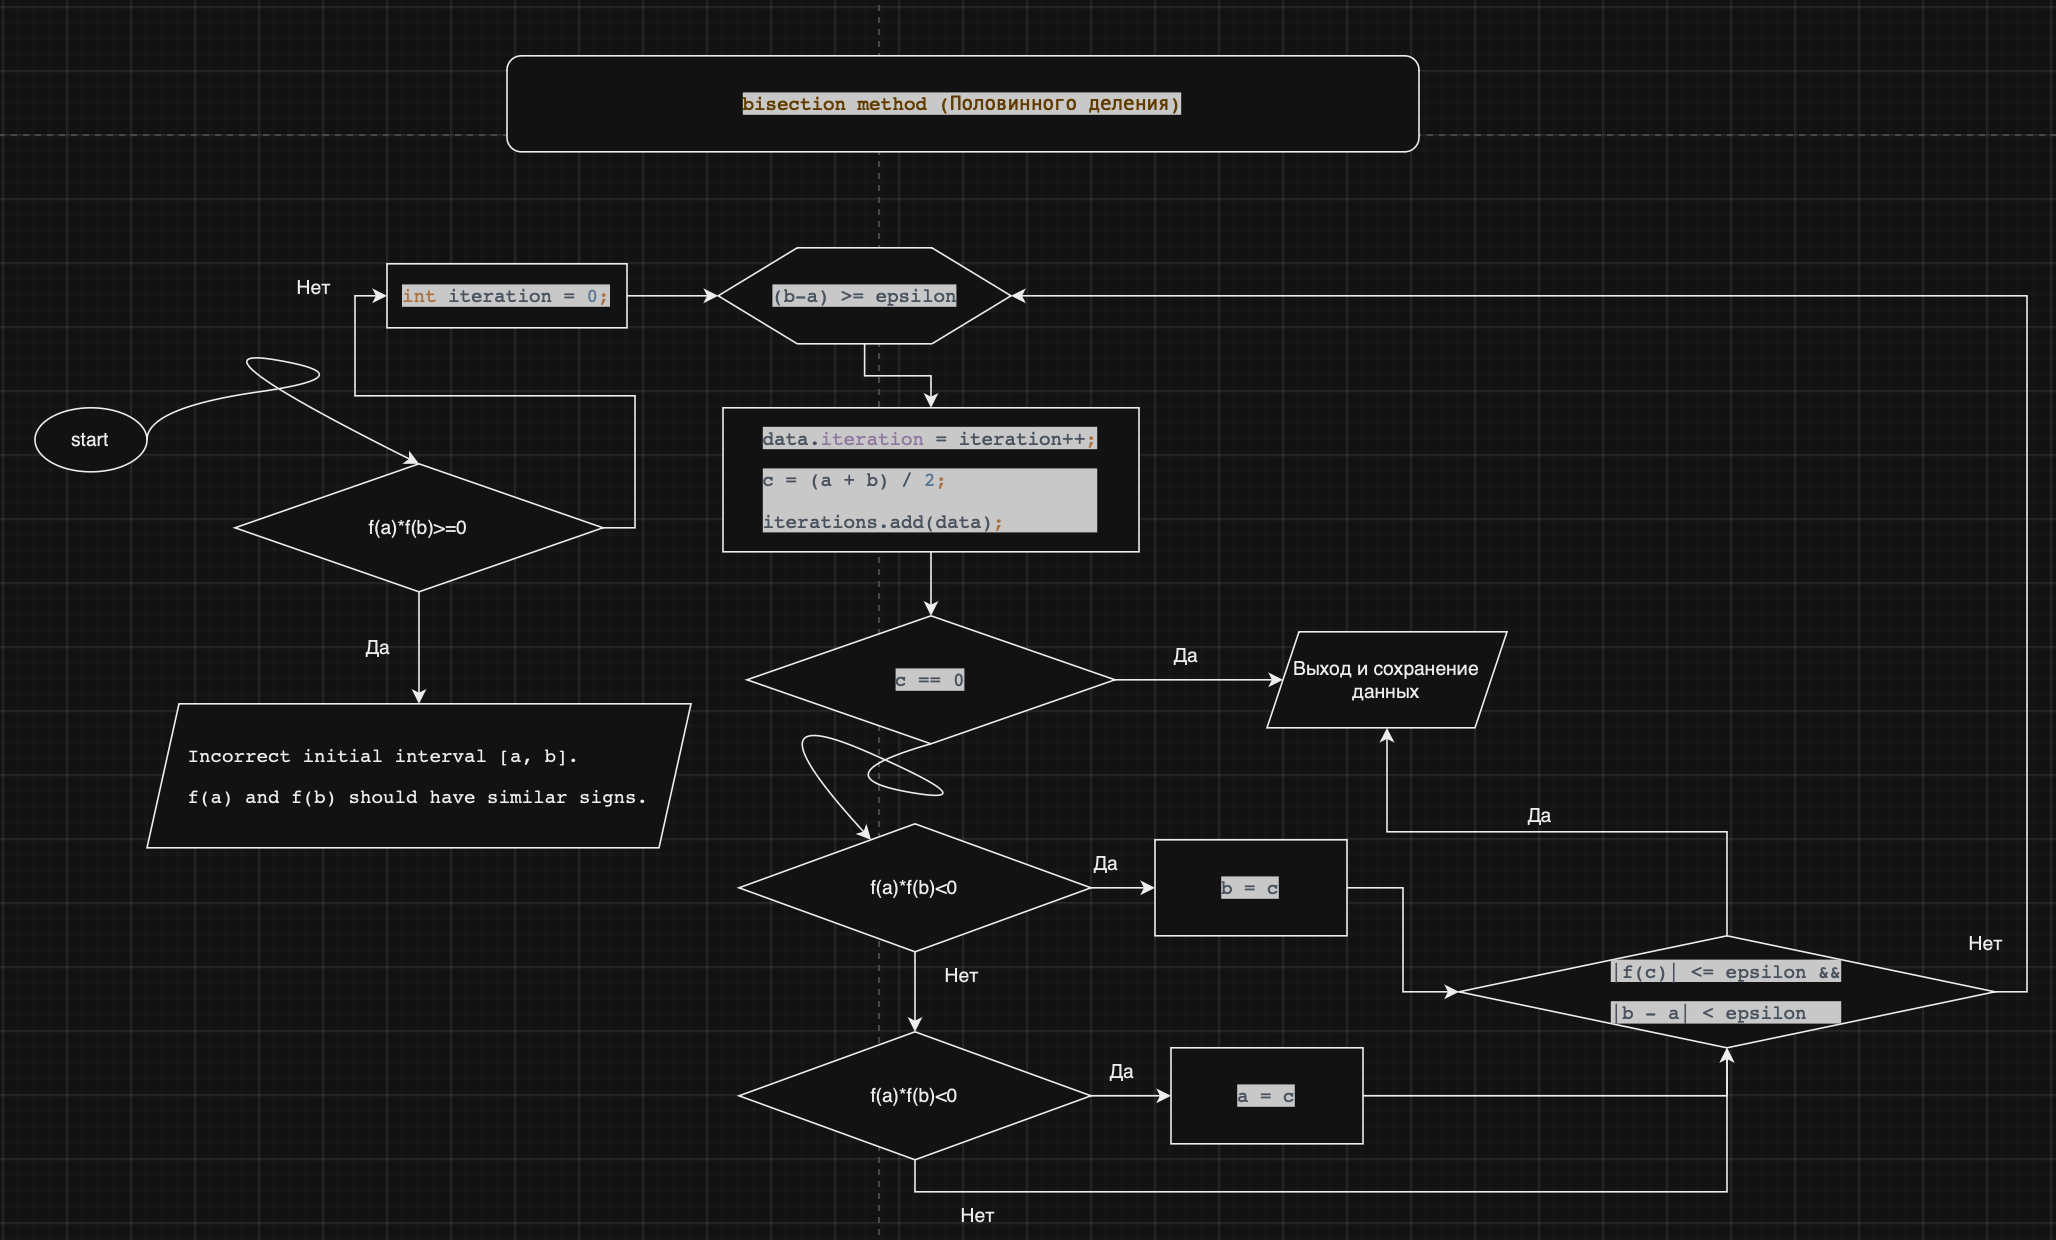
\includegraphics[width=.7\textwidth]{bisection.png}
\\ \\
Реализация кода:
\\ \\
\begin{lstlisting}[frame=single, basicstyle=\ttfamily, breaklines=true, breakatwhitespace=true, postbreak=\mbox{\textcolor{red}{$\hookrightarrow$}\space}]
    public static String bisection(Coordinates coordinates) {
        double a = coordinates.getA();
        double b = coordinates.getB();
        double epsilon = coordinates.getEps();
        List<IterationsForBisection> iterations = new ArrayList<>();

        if (coordinates.getValue(a) * coordinates.getValue(b) >= 0) {
            System.out.println("Incorrect initial interval [a, b]. f(a) and f(b) should have similar signs.");
            return "Incorrect initial interval [a, b]. f(a) and f(b) should have similar signs.";
        }

        int iteration = 0;

        double c = a;
        while ((b-a) >= epsilon) {
            IterationsForBisection data = new IterationsForBisection();
            data.iteration = iteration++;
            data.a = a;
            data.b = b;
            // Find middle point
            c = (a + b) / 2;
            data.x = c;
            data.fA = coordinates.getValue(a);
            data.fB = coordinates.getValue(b);
            data.fX = coordinates.getValue(c);
            data.absAB = Math.abs(a-b);
            iterations.add(data);
            if (coordinates.getValue(c) == 0.0)
                break;
            else if (coordinates.getValue(c) * coordinates.getValue(a) < 0)
                b = c;
            else
                a = c;
            if (Math.abs(coordinates.getValue(c)) <= epsilon && Math.abs(b - a) < epsilon)
                break;
        }
        Gson gson = new Gson();
        try (FileWriter writer = new FileWriter("tmp.json")) {
            writer.write(gson.toJson(iterations));
        } catch (IOException e) {
            e.printStackTrace();
        }
        System.out.printf("The root is %.6f\n", c);
        return "The root is " + c+ "; f(x) = "+coordinates.getValue(c)+"; iter: "+iteration;
    }
\end{lstlisting}

2. Метод Ньютона
\\ \\
Диаграмма:\\
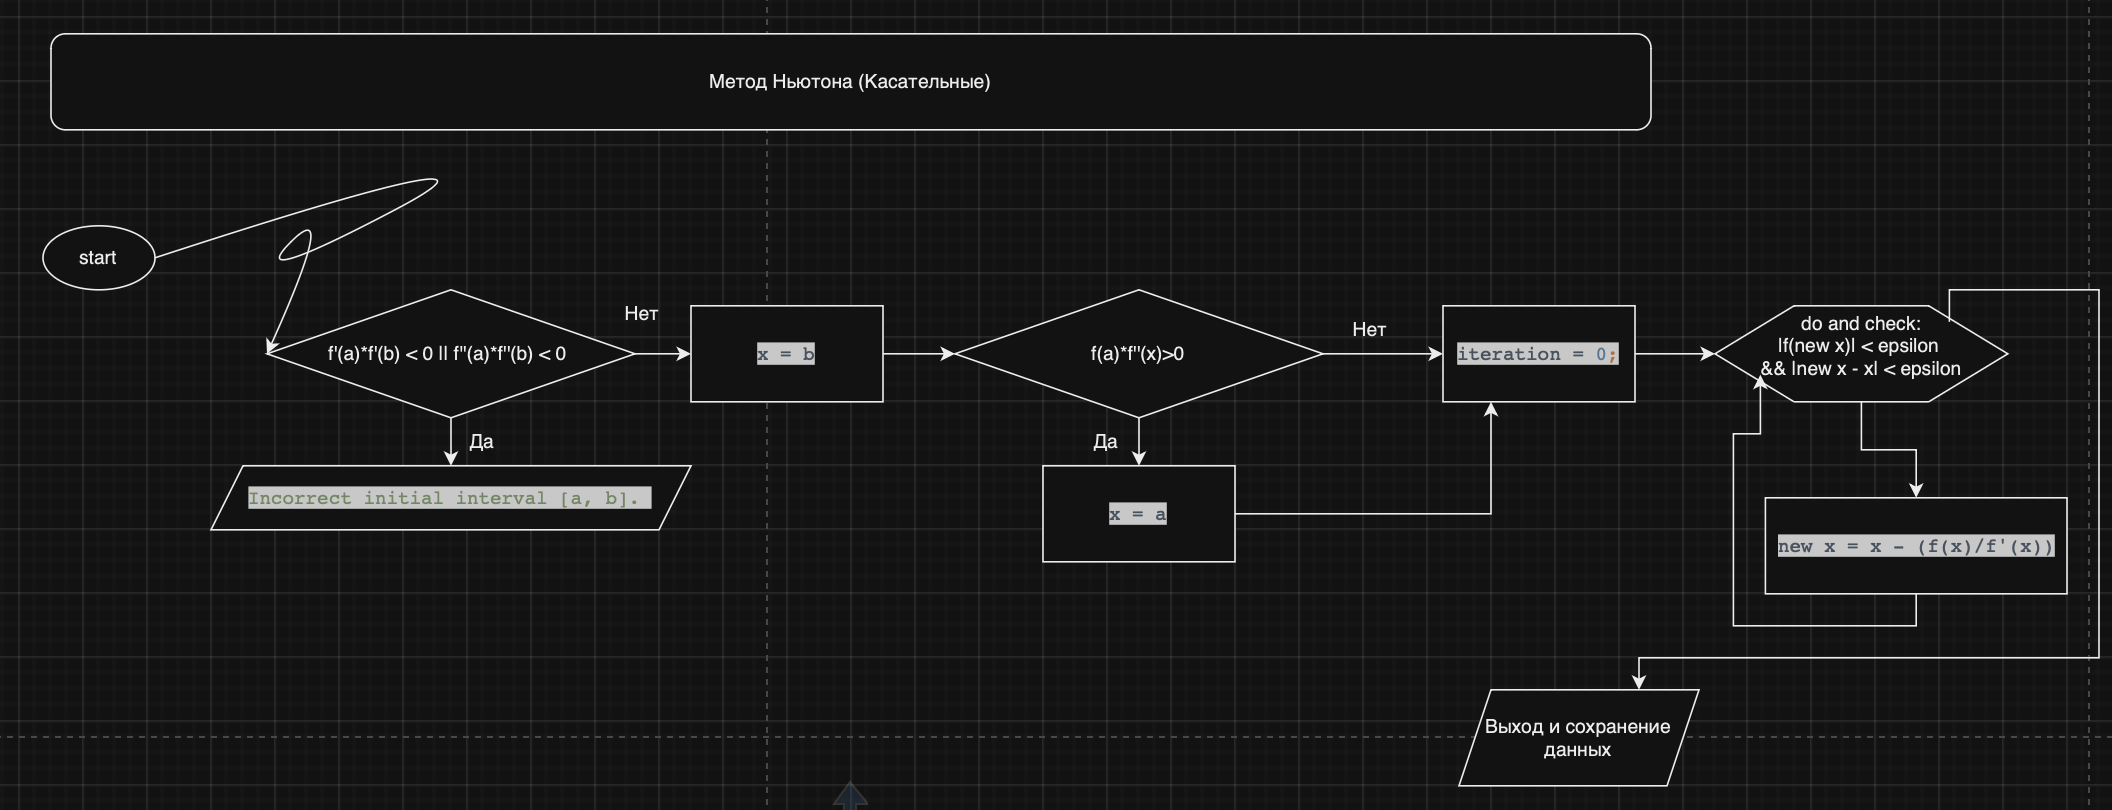
\includegraphics[width=.7\textwidth]{newtown.png}
\\ \\
Реализация кода:
\\ \\
\begin{lstlisting}[frame=single, basicstyle=\ttfamily, breaklines=true, breakatwhitespace=true, postbreak=\mbox{\textcolor{red}{$\hookrightarrow$}\space}]
    public static String newtown(Coordinates coordinates) {
        double a = coordinates.getA();
        double b = coordinates.getB();
        double epsilon = coordinates.getEps();
        List<IterationsForNewt> iterations = new ArrayList<>();

        // Check the initial interval conditions for the derivatives
        if ((coordinates.getDev(1, a) * coordinates.getDev(1, b) < 0) || (coordinates.getDev(2, a) * coordinates.getDev(2, b) < 0)) {
            System.out.println("Incorrect initial interval [a, b]. f'(a) and f'(b) or f''(a) and f''(b) should have opposite signs.");
            return "Incorrect initial interval [a, b]. f'(a) and f'(b) or f''(a) and f''(b) should have opposite signs.";
        }

        double x = b;
        if (coordinates.getValue(a) * coordinates.getDev(2, a) > 0) {
            x = a;
        }

        double newX;
        int iteration = 0;
        int maxIterations = 1000;

        do {
            IterationsForNewt data = new IterationsForNewt();
            data.iteration = iteration++;
            data.xi = x;
            data.f_xi = coordinates.getValue(x);
            data.f1_xi = coordinates.getDev(1, x);

            if (Math.abs(data.f1_xi) < epsilon) {
                System.out.println("Division by zero in derivative.");
                return "Division by zero in derivative.";
            }

            newX = x - (data.f_xi / data.f1_xi);
            data.x_2i = newX;
            data.absX = Math.abs(newX - x);

            iterations.add(data);

            if (Math.abs(coordinates.getValue(newX)) < epsilon && Math.abs(newX - x) < epsilon) {
                break;
            }

            x = newX;

            if (iteration > maxIterations) {
                System.out.println("Max iterations reached without convergence.");
                return "Max iterations reached without convergence.";
            }

        } while (true);

        System.out.printf("The root is %.6f\n", x);
        Gson gson = new Gson();
        try (FileWriter writer = new FileWriter("tmp.json")) {
            writer.write(gson.toJson(iterations));
        } catch (IOException e) {
            e.printStackTrace();
        }

        return "The root is " + x+ "; f(x) = "+coordinates.getValue(x)+"; iter: "+iteration;
    }
\end{lstlisting}
3. Метод простой итерации
\\ \\
Диаграмма:\\
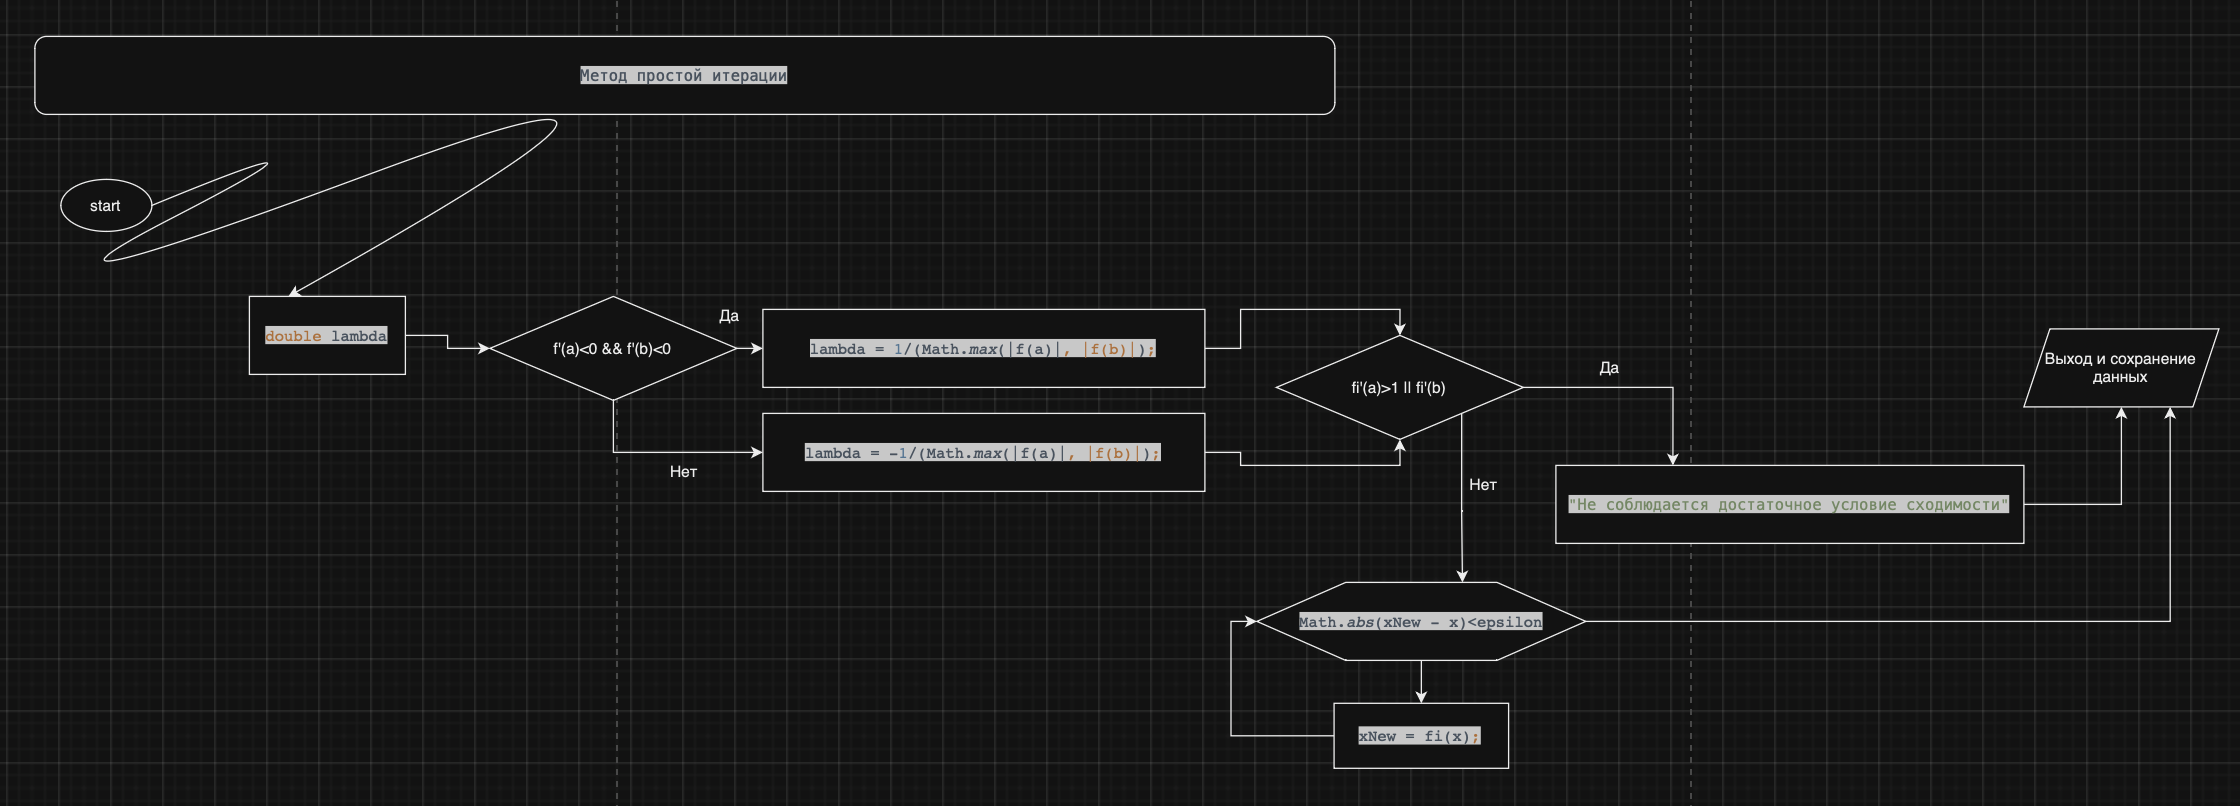
\includegraphics[width=.7\textwidth]{simple.png}
\\ \\
Реализация кода:
\\ \\
\begin{lstlisting}[frame=single, basicstyle=\ttfamily, breaklines=true, breakatwhitespace=true, postbreak=\mbox{\textcolor{red}{$\hookrightarrow$}\space}]
    Coordinates coordinates1;
    private double fi(double x, double lambda){
        return x+lambda*coordinates1.getValue(x);
    }
    public double fiDev(double point, double lambda) {
        return (fi(point + 0.0001, lambda) - fi(point - 0.0001, lambda)) / (2 * 0.0001);
    }
    public String simple(Coordinates coordinates) {
        coordinates1 = coordinates;
        double a = coordinates.getA();
        double b = coordinates.getB();
        double epsilon = coordinates.getEps();
        List<IterationsForSimple> iterations = new ArrayList<>();
        double lambda;
        if(coordinates.getDev(1, a)<0 && coordinates.getDev(1, b)<0){
            lambda = 1/(Math.max(Math.abs(coordinates.getDev(1, a)), Math.abs(coordinates.getDev(1, b))));
        }else{
            lambda = -1/(Math.max(Math.abs(coordinates.getDev(1, a)), Math.abs(coordinates.getDev(1, b))));
        }

        if(fiDev(a, lambda)>1 || fiDev(b, lambda)>1){
            System.out.println("-");
            return "-";
        }

        double x = a;
        int iteration = 0;
        while (true){
            IterationsForSimple data = new IterationsForSimple();
            data.iteration = iteration++;
            data.x = x;
            double xNew = fi(x, lambda);
            data.xNew = xNew;
            data.fi = fi(xNew, lambda);
            data.f = coordinates.getValue(xNew);
            data.absX = Math.abs(xNew - x);
            if(Math.abs(xNew - x)<epsilon){
                break;
            }
            x = xNew;
            iterations.add(data);
        }

        System.out.printf("The root is %.6f\n", x);

        Gson gson = new Gson();
        try (FileWriter writer = new FileWriter("tmp.json")) {
            writer.write(gson.toJson(iterations));
        } catch (IOException e) {
            e.printStackTrace();
        }

        return "The root is " + x+ "; f(x) = "+coordinates.getValue(x)+"; iter: "+iteration;
    }
\end{lstlisting}
4. Метод простой итерации для систем
\\ \\
Диаграмма:\\
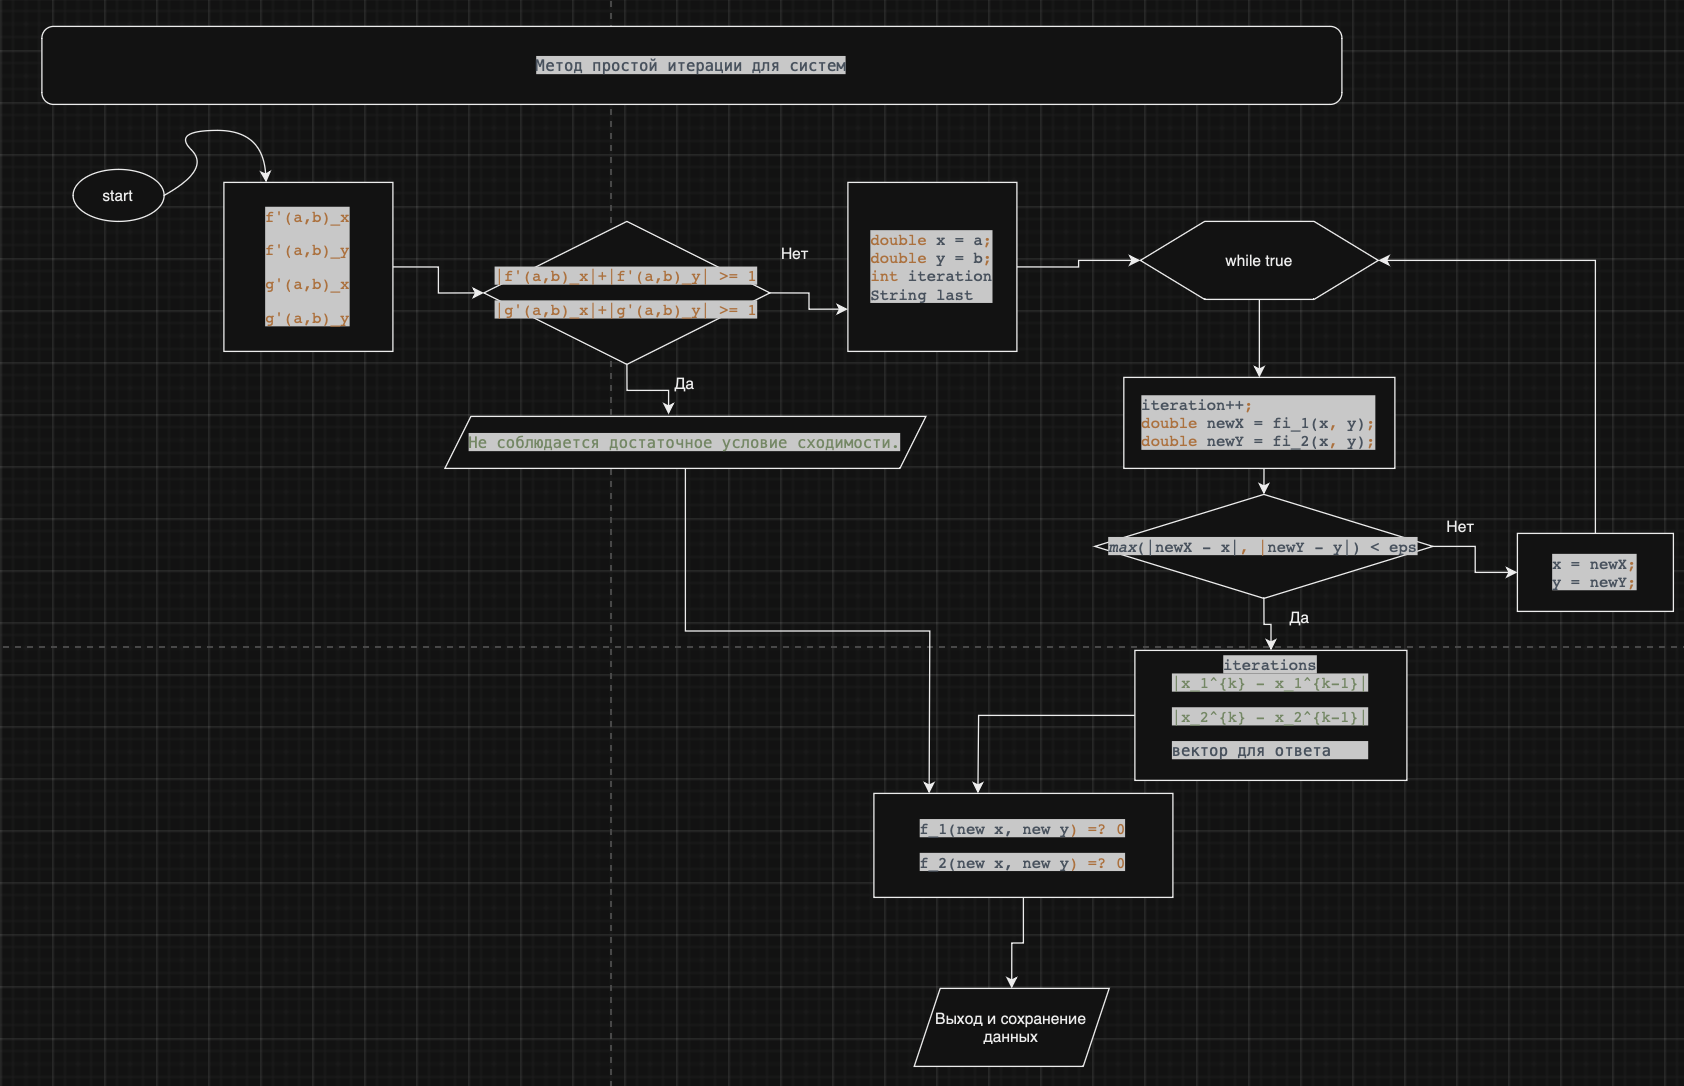
\includegraphics[width=.7\textwidth]{simpleSis.png}
\\ \\
Реализация кода:
\\ \\
\begin{lstlisting}[frame=single, basicstyle=\ttfamily, breaklines=true, breakatwhitespace=true, postbreak=\mbox{\textcolor{red}{$\hookrightarrow$}\space}]
    public static String simpl(Coordinates coordinates) {
        double a = coordinates.getA();
        double b = coordinates.getB();
        double epsilon = coordinates.getEps();
        IterationsForSis iterations = new IterationsForSis();
        double pdv11 = coordinates.getFiSisPdv(a, b, 1);
        double pdv12 = coordinates.getFiSisPdv(a, b, 2);
        double pdv21 = coordinates.getFiSisPdv(a, b, 3);
        double pdv22 = coordinates.getFiSisPdv(a, b, 4);

        if ((Math.abs(pdv11)+Math.abs(pdv12)>=1) || (Math.abs(pdv21)+Math.abs(pdv22)>=1)) {
            System.out.println("Incorrect initial [a, b].");
            return "Incorrect initial [a, b].";
        }

        double x = a;
        double y = b;
        int iteration = 0;
        String last;
        while (true) {
            iteration++;
            double newX = coordinates.getFiSis(x, y, 1);
            double newY = coordinates.getFiSis(x, y, 2);

            // Check for convergence criteria
            if ((Math.max(Math.abs(newX - x), Math.abs(newY - y)) < epsilon)||(iteration>100)){
                iterations.absX = Math.abs(newX - x);
                iterations.absY = Math.abs(newY - y);
                iterations.iteration = iteration;
                iterations.xAnswer = newX;
                iterations.yAnswer = newY;
                last = "|x_1^{k} - x_1^{k-1}| = "+Math.abs(newX - x)+ "; |x_2^{k} - x_2^{k-1}| = "+Math.abs(newY - y);
                break;
            }
            x = newX;
            y = newY;
        }
        Gson gson = new Gson();
        try (FileWriter writer = new FileWriter("tmp.json")) {
            writer.write(gson.toJson(iterations));
        } catch (IOException e) {
            e.printStackTrace();
        }
        System.out.println("The root is x:"+x+" y: "+y);
    }
\end{lstlisting}
\section{Ссылка на GitHub с основной реализацией}
https://github.com/Alex-de-bug/cm\_math/
\section{Вывод}
    В данной работе мы изучили некоторые методы для решения линейных уравнений и нелинейных. Первую часть мы сделали руками, чтобы понять детально методы. Далее мы реализовали некоторые из методов кодом.
\end{document}

\[
    3x^3+1,7x^2-15,42x+6,89\]

\begin{lstlisting}[frame=single, basicstyle=\ttfamily, breaklines=true, breakatwhitespace=true, postbreak=\mbox{\textcolor{red}{$\hookrightarrow$}\space}]
    
\end{lstlisting}
\section{Ссылка на GitHub с основной реализацией}
https://github.com/Alex-de-bug/cm\_math/tree/main/lab1
\section{Пример работы программы}
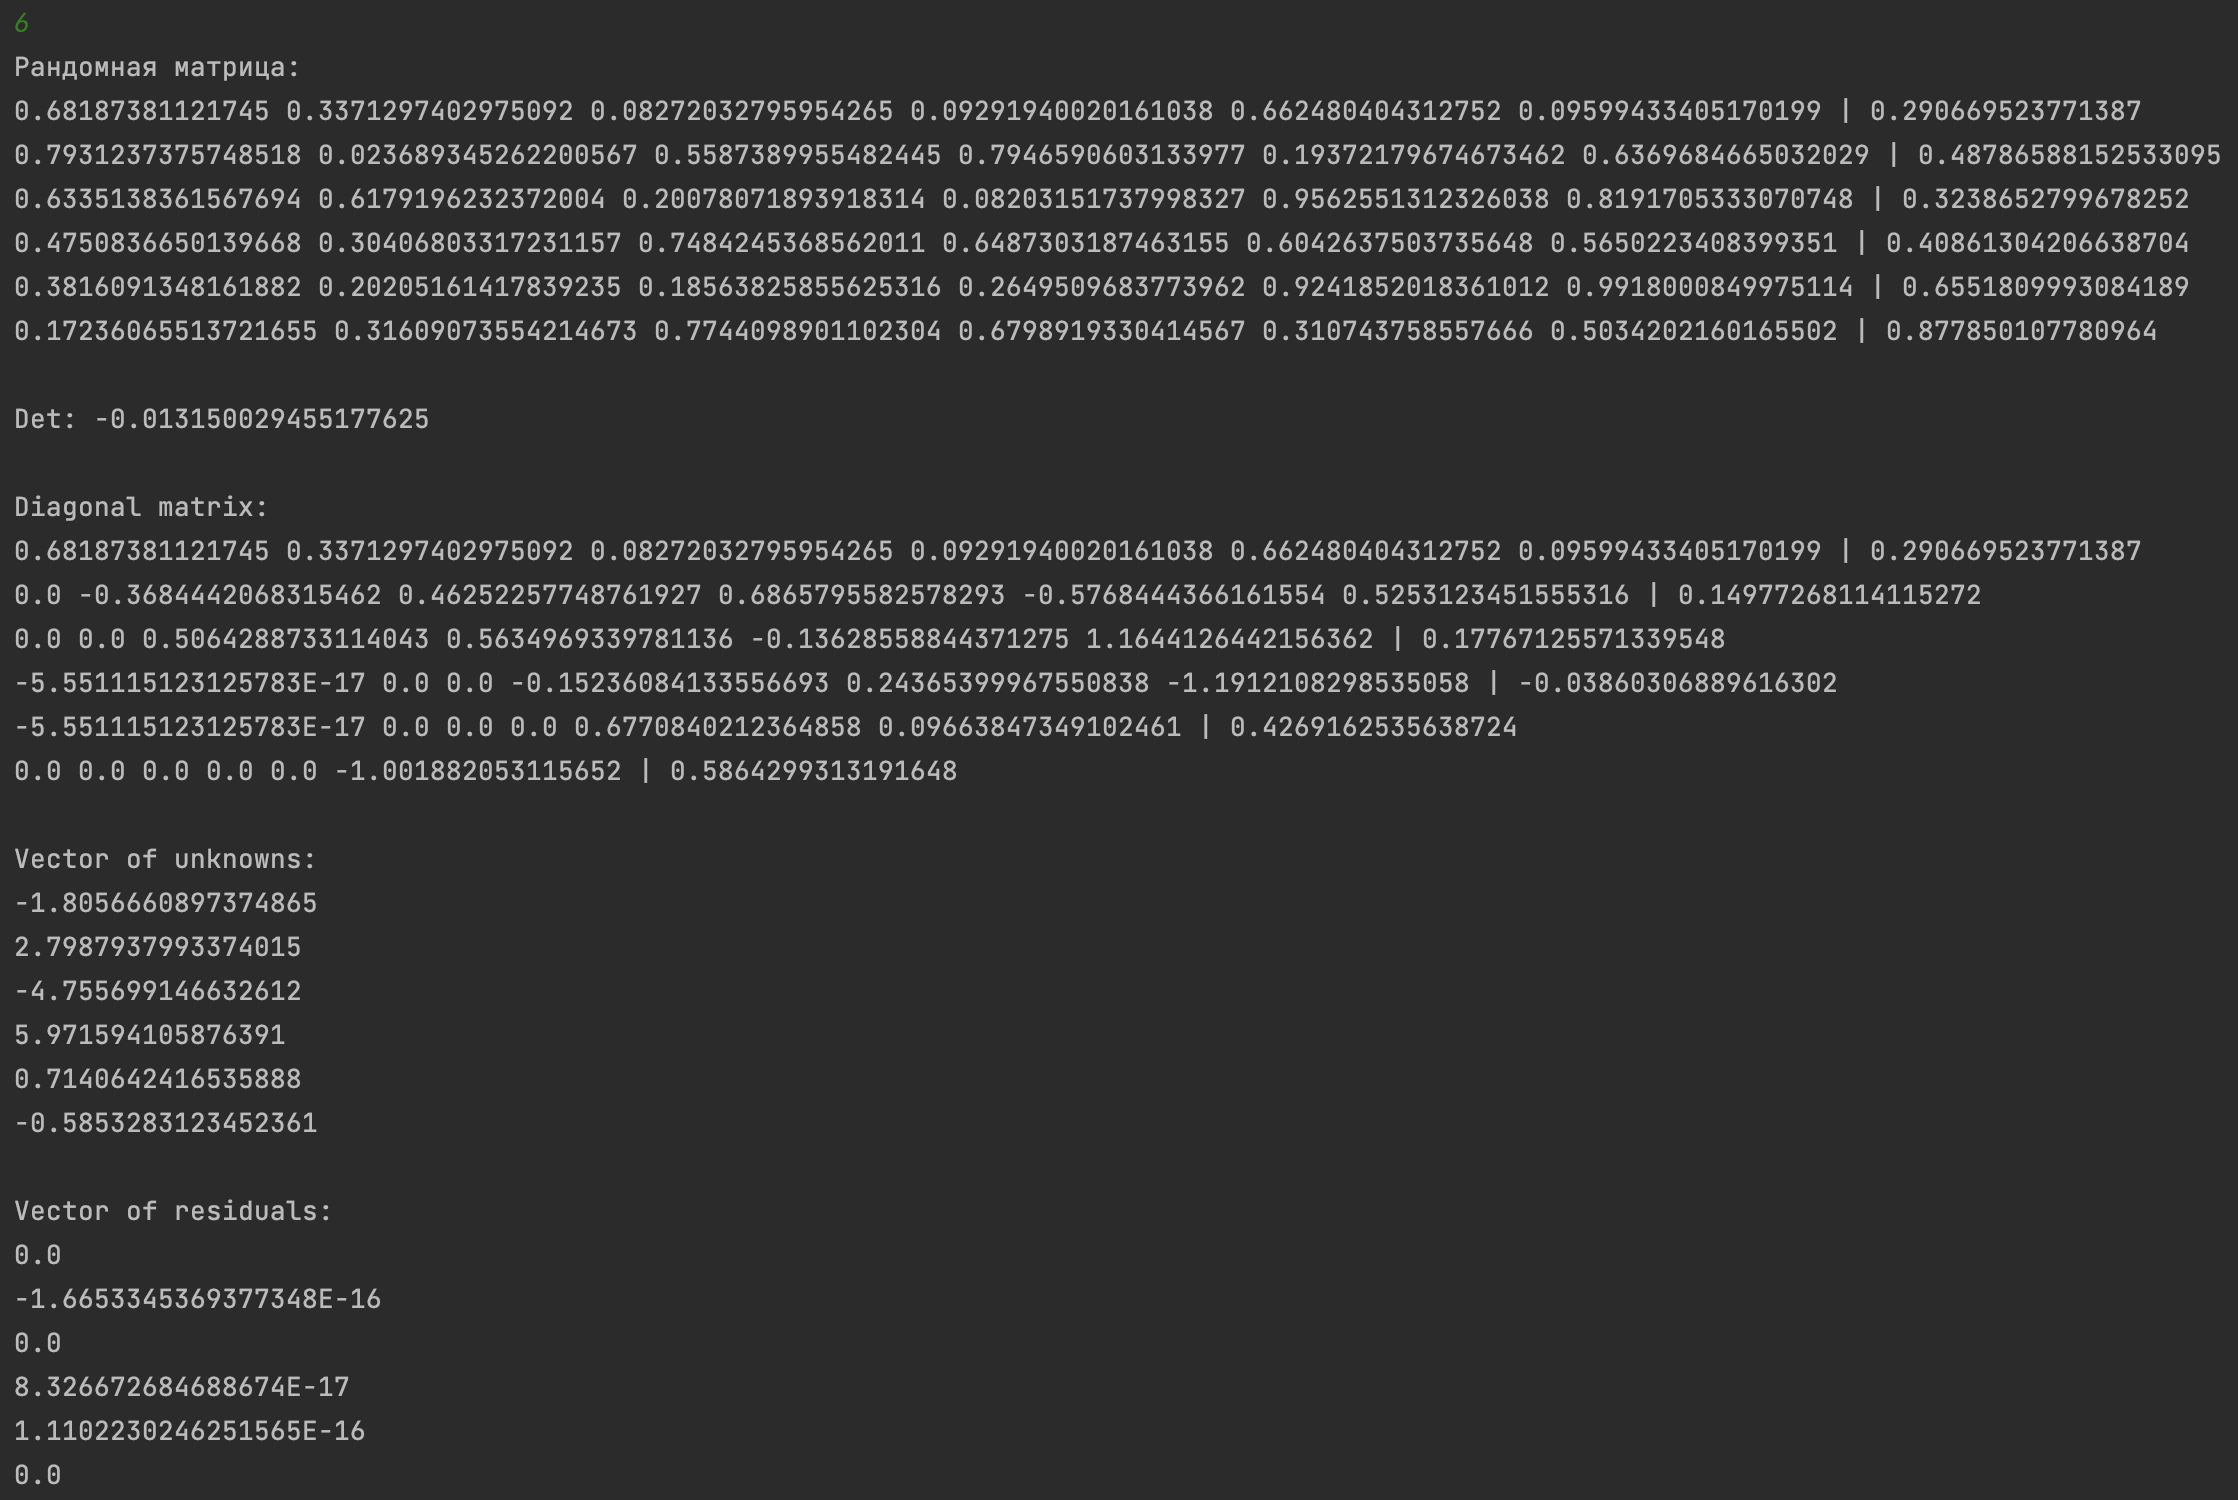
\includegraphics[width=1\textwidth]{3}